\documentclass[tikz, preview=true, border=2mm]{standalone}

\definecolor{Blue}{HTML}{fa7303}
\definecolor{Orange}{HTML}{0e0441}

\renewcommand*\familydefault{\sfdefault}

\usepackage{tikz}
\usetikzlibrary{mindmap,trees,shadows}

\begin{document}

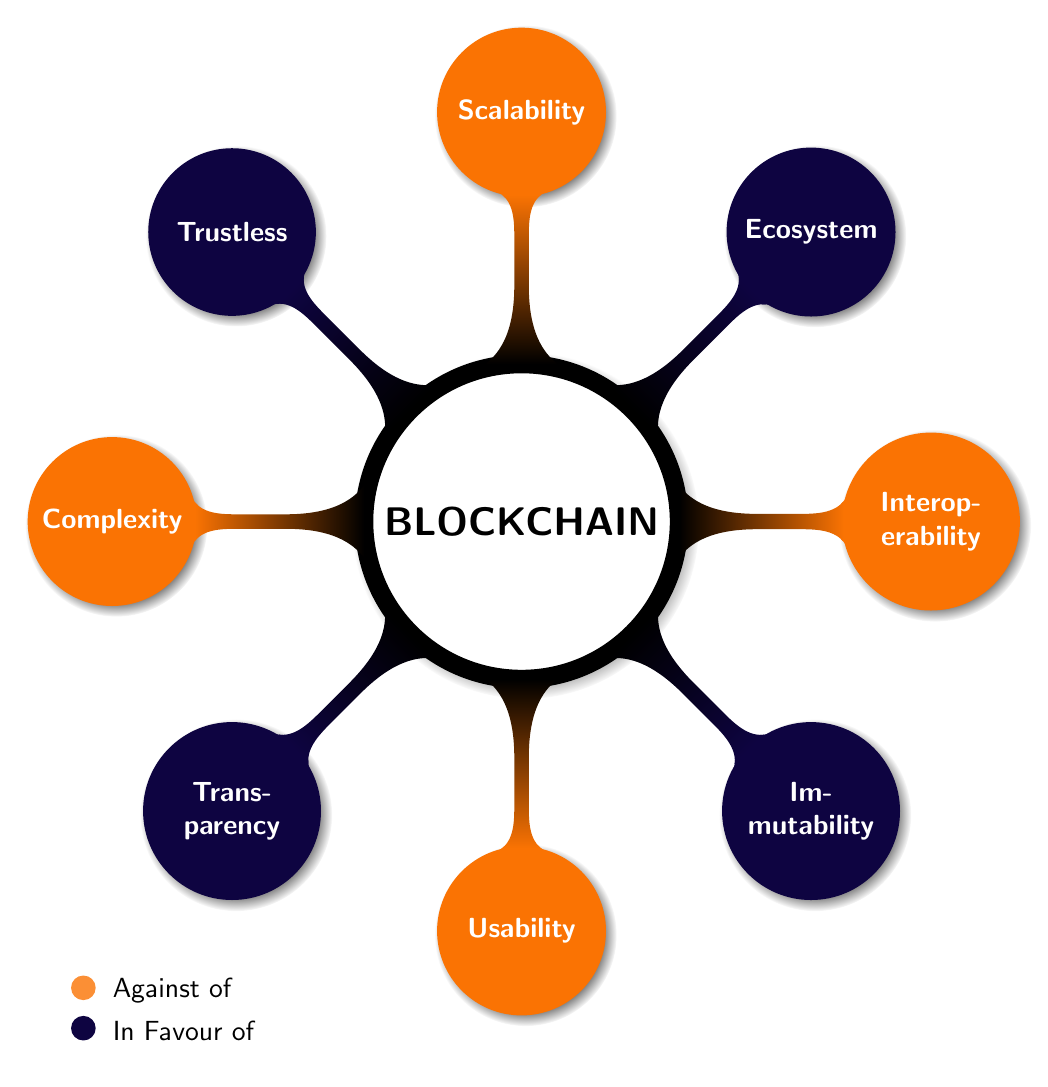
\begin{tikzpicture}
    [decoration={start radius=1cm, end radius=.5cm,amplitude=3mm,angle=30}]

    \begin{scope}[mindmap,
        every node/.style={concept, circular drop shadow, minimum size=0pt,execute at begin node=\hskip0pt, font=\bfseries},
        root concept/.append style={
        concept color=black, fill=white, line width=1.5ex, text=black, font=\Large\scshape\bfseries,},
        level 1 concept/.append style={font=\bfseries},
        text=white,
        partner/.style={},
        grow cyclic,
        level 1/.append style={level distance=5.2cm,sibling angle=45}]
        
        \node [root concept] (team) {BLOCKCHAIN}[rotate=202.5] % root
        child [partner, style={concept color=Orange}] { node {Ecosystem}
        }
        child [partner, style={concept color=Blue}] { node {Scalability}
        }
        child [partner, style={concept color=Orange}] { node {Trustless}
        }
        child [partner, style={concept color=Blue}] { node {Complexity}
        }
        child [partner, style={concept color=Orange}] { node {Transparency}
        }
        child [partner, style={concept color=Blue}] { node {Usability}
        }
        child [partner, style={concept color=Orange}] { node {Immutability}
        }
        child [partner, style={concept color=Blue}] { node {Interoperability}
        };
        % child [partner, style={concept color=Orange}] { node {Sharing}
        % }
    \end{scope}

    \begin{scope}[xshift=-4.5cm, yshift=-6.2cm,every node/.style={align=left,text=black}]
        \matrix[row sep=0pt,column sep=1mm, align=left, nodes={align=left, anchor=west}] {
        \fill [Blue!80] (0,.25ex) circle (1ex); & \node{Against of};\\
        \fill [Orange] (0,.25ex) circle (1ex); & \node{In Favour of};\\
        };
    \end{scope}
\end{tikzpicture}

\end{document}